\subsection{Tree Traversal}
\label{sec:traversal}
% At each step you reason about tradeoffs/alternative design choices and
% justify why you did it in the way you did it (advantages/shortcommings,
% and why your approach is reasonable). Of course mostly related to performance.

% Whenever possible, support your reasoning with (as in point to) experimental
% evaluation results (next).

% \begin{itemize}
% 	\item using an integer to represent the stack
% 	\item the first traversal logic (show figure)
% 	\item the continuous traversal logic (show figure)
% 	\item checking a median on one dimension
% 	\item checking all medians from all dimensions (show equation)
% 	\item 
% 	\item 
% 	\item 
% \end{itemize}	

%   3.3 Tree Traversal
%     - explaining the solution to use a stack 
%     - showing a figure of the first traversal: first go to the leaf in which the query naturally belongs, there is a unique leaf to which it naturally belongs to 
%     - showing (2-3) figures of the continuous traversal with a stack

%     3.3.1 Representing the Stack as an Integer
%       - including an equation that shows the bit arithmetic of setVisited

%     3.3.2 Validating Whether to Look at the `second`
%       - reasoning about the original median check
%       - showing and reasoning about Cosmin's equation
%       - comparing the two
%         - benefits, trade-offs


% As mention in the Background, Futhark does not support recursion, which is why the pseudo-code from Algorithm 3 is rewritten into an imperative version. One such solution is using a stack to traverse the tree incrementally while deciding which nodes to visit next. The figure below demonstrates the traverse down to the first leaf; this example does not need a stack because, at this point, we do not know if we need to visit additional leaves. Figures X-X show the traversal continuing from the first leaf, in which a stack is necessary. 
% Divide and conquer recursion is difficult to map, especially efficiently for parallel execution. Due to divergence and various irregular things.  



In section \ref{sec:back} the tree traversal Algorithm \ref{alg:tree}, is created using recursion, and as in section \ref{sec:kdtree} we must re-write the traversal without recursion. The proposed solution uses a stack, and the stack is represented as an integer, since the height of the tree never exceeds 32. 
\\[2mm]
The traversal has two stages overall stages: (1) the first traversal finding the unique leaf in which the query naturally belongs, (2) backtracking the tree to find additional or better KNNs. 

\subsubsection{The First Traversal}

As described in section \ref{sec:back}, first denotes the child of the current node that is on the same side as median w.r.t the query, similarly second denotes the child of the current node that is on the opposite side of the median. 
Figure \ref{fig:t1} demonstrates how the tree is traversed to the leaf in which the query belongs, note that the leaf marked with red is denoted first and its sibling leaf is denoted second. 

\begin{figure}[H]
\centering
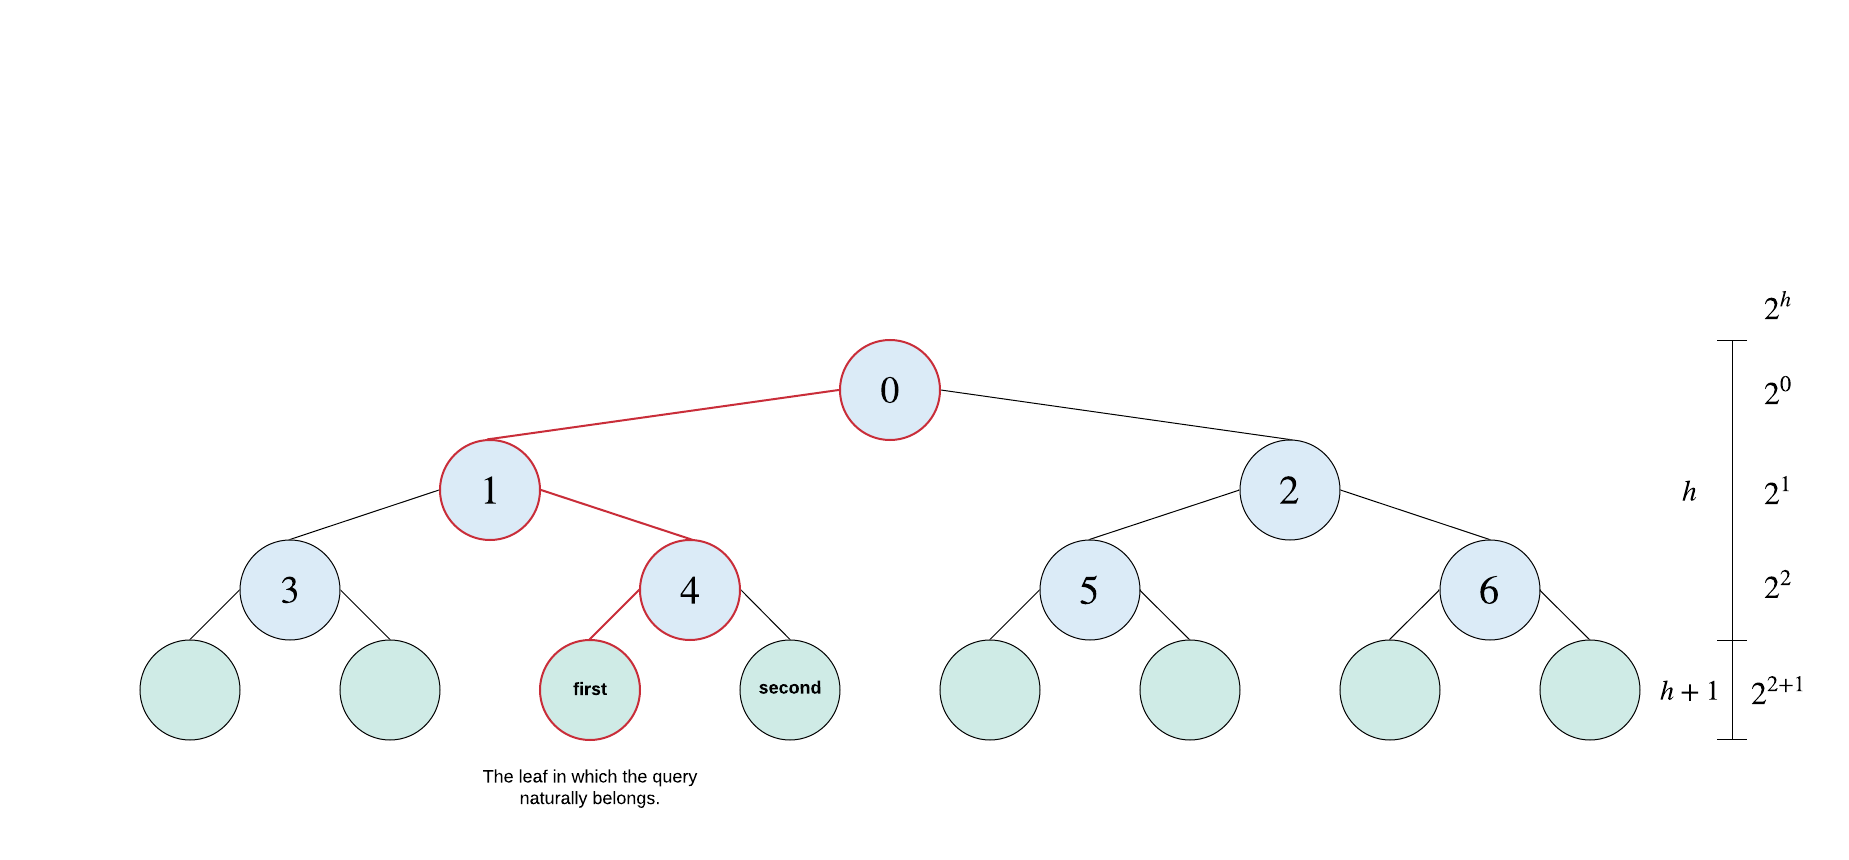
\includegraphics[width=1\textwidth]{pics/kd-tree-visual/22.png}
\caption{The first traversal finding the leaf in which the query naturally belongs.}
\label{fig:t1}
\end{figure}

% \begin{listing}[H]
% \begin{minted}{haskell}
% entry firstTraverse [d][q] (height:   i32)  (median_dims: [q]i32)
%                            (query: [d]f32)  (median_vals: [q]f32) =

%     let new_leaf = loop node_index = 0
%         while !(isLeaf height node_index) do
%           if query[median_dims[node_index]] <= median_vals[node_index]
%           then (node_index+1)*2-1
%           else (node_index+1)*2

%     in new_leaf
% \end{minted}
% \caption{Futhark implementation of the first tree traversal.}
% \label{lst:first}
% \end{listing}


\subsubsection{The Traversal for Additional Leaves}


In this demonstration, we look at a fictive traversal in which we always check the second node. The validation technique as to whether to check the second node or not, is elaborated in section \ref{sec:valid}. 
\\[2mm]
Figure \ref{fig:t2} is a continuation of figure \ref{fig:t1}, in which the initial leaf is reached and the stack is popped to see if the second node has been visited or not. Since it had not been visited, the traversal also visits the second node. 

% \begin{figure}[H]
% \centering
% 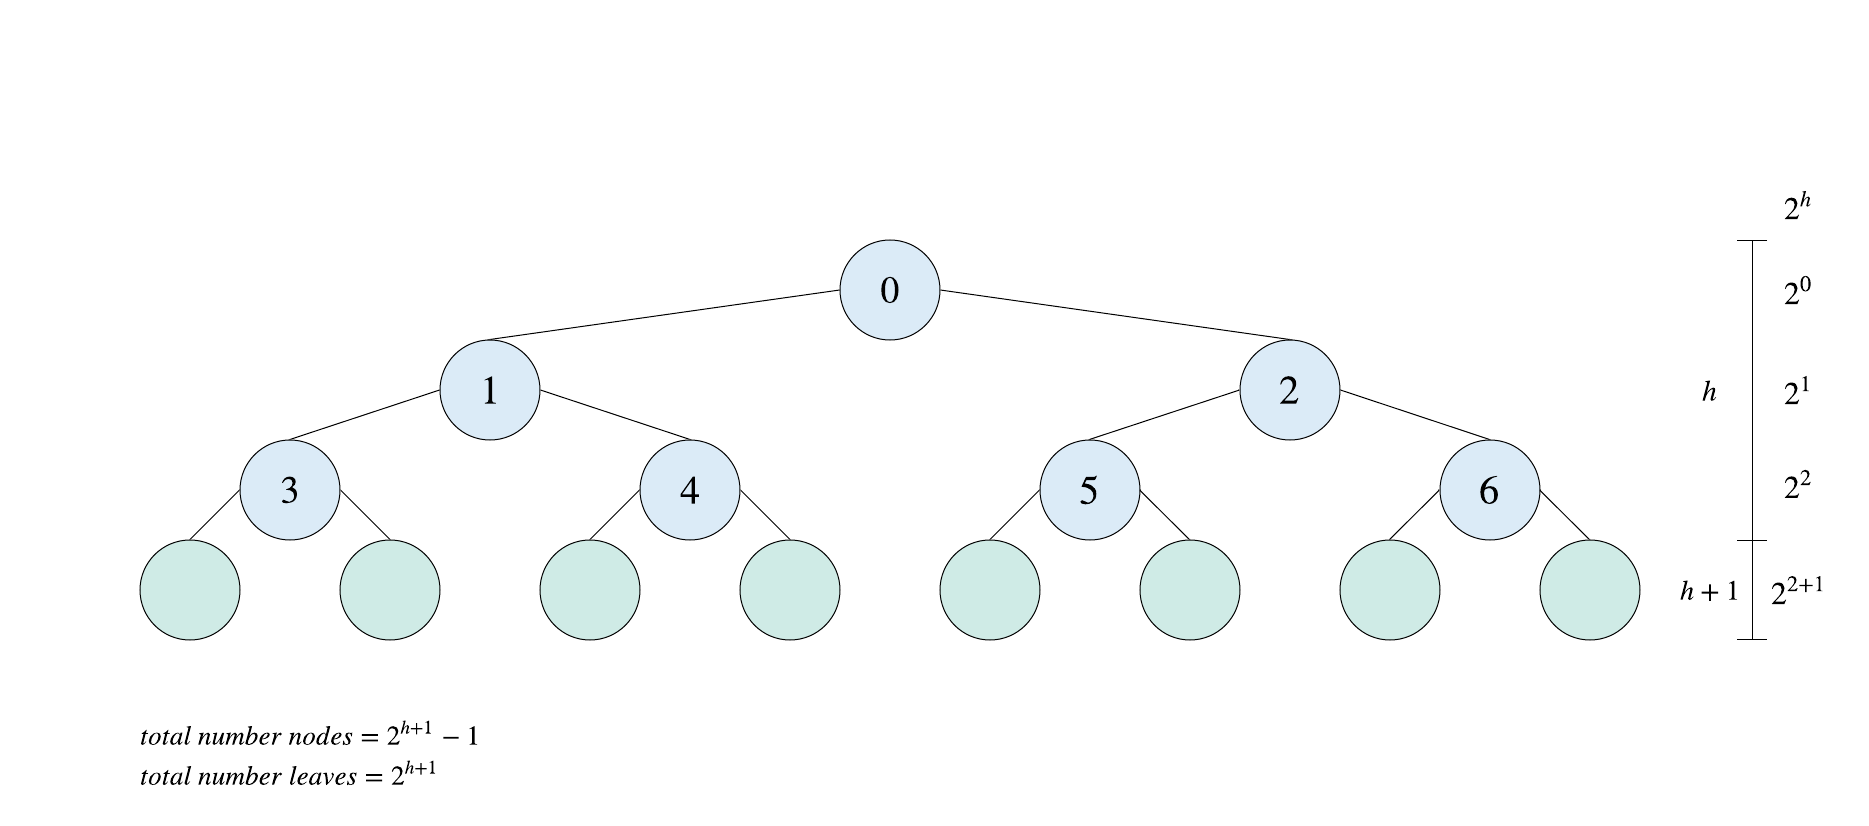
\includegraphics[width=0.9\textwidth]{pics/kd-tree-visual/1.png}
% \caption{}
% \end{figure}


% \begin{figure}[H]
% \centering
% 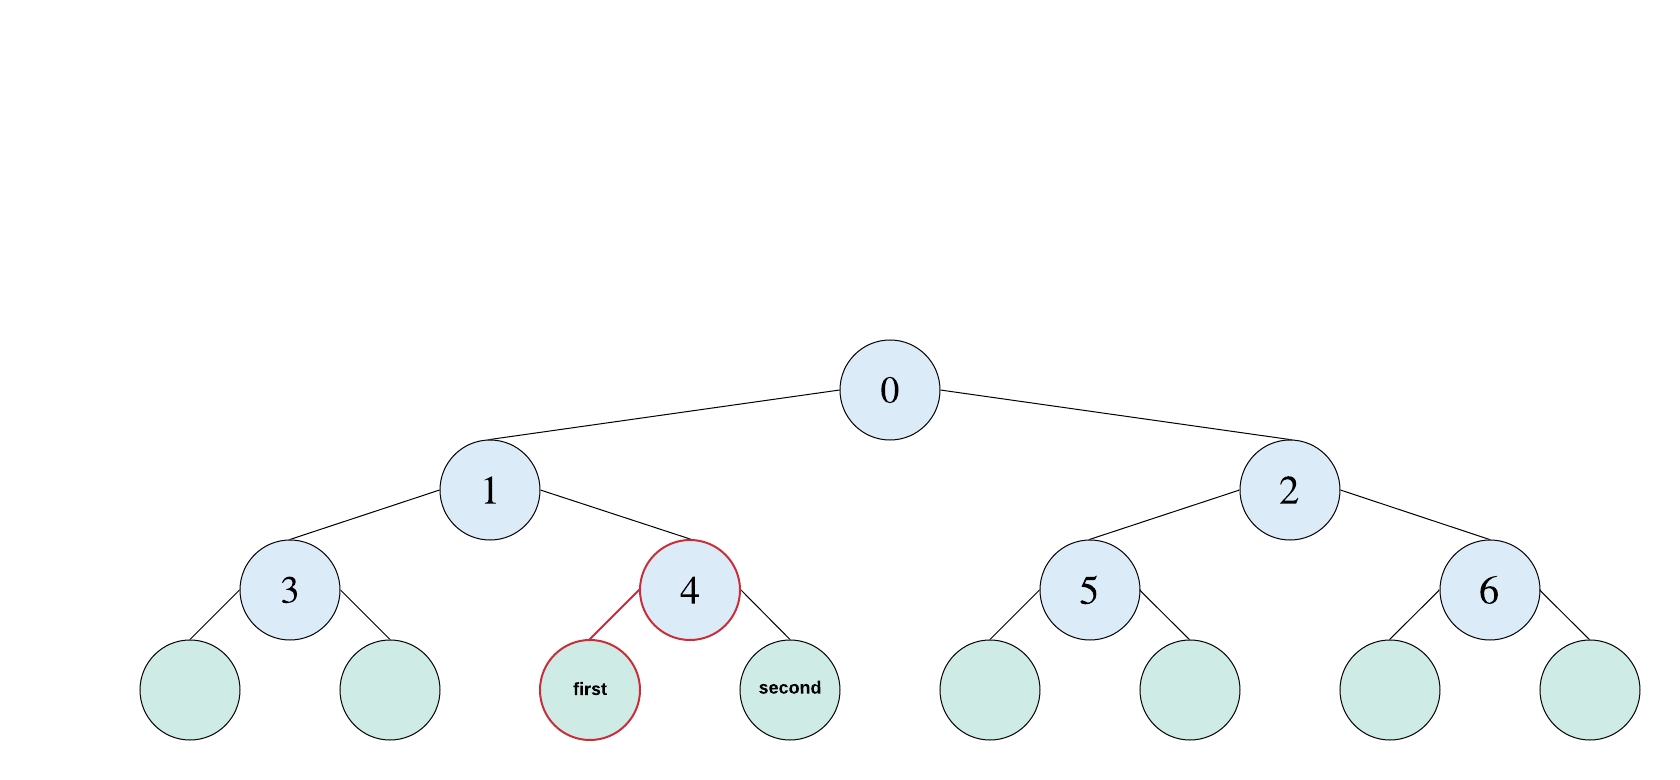
\includegraphics[width=0.9\textwidth]{pics/kd-tree-visual/3.png}
% \caption{}
% \end{figure}

% \begin{figure}[H]
% \centering
% 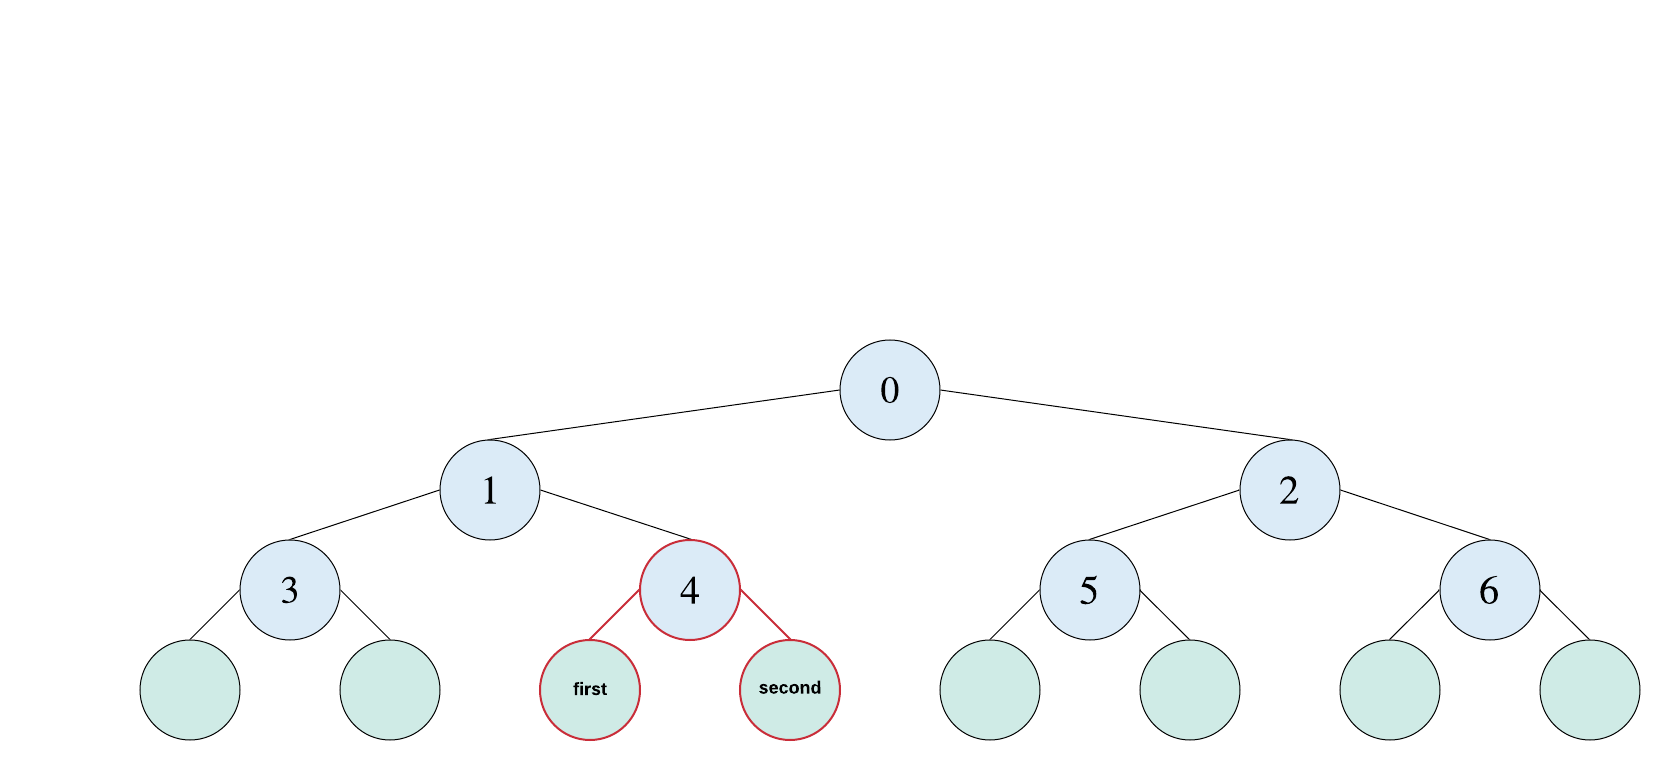
\includegraphics[width=0.9\textwidth]{pics/kd-tree-visual/4.png}
% \caption{}
% \end{figure}

\begin{figure}[H]
\centering
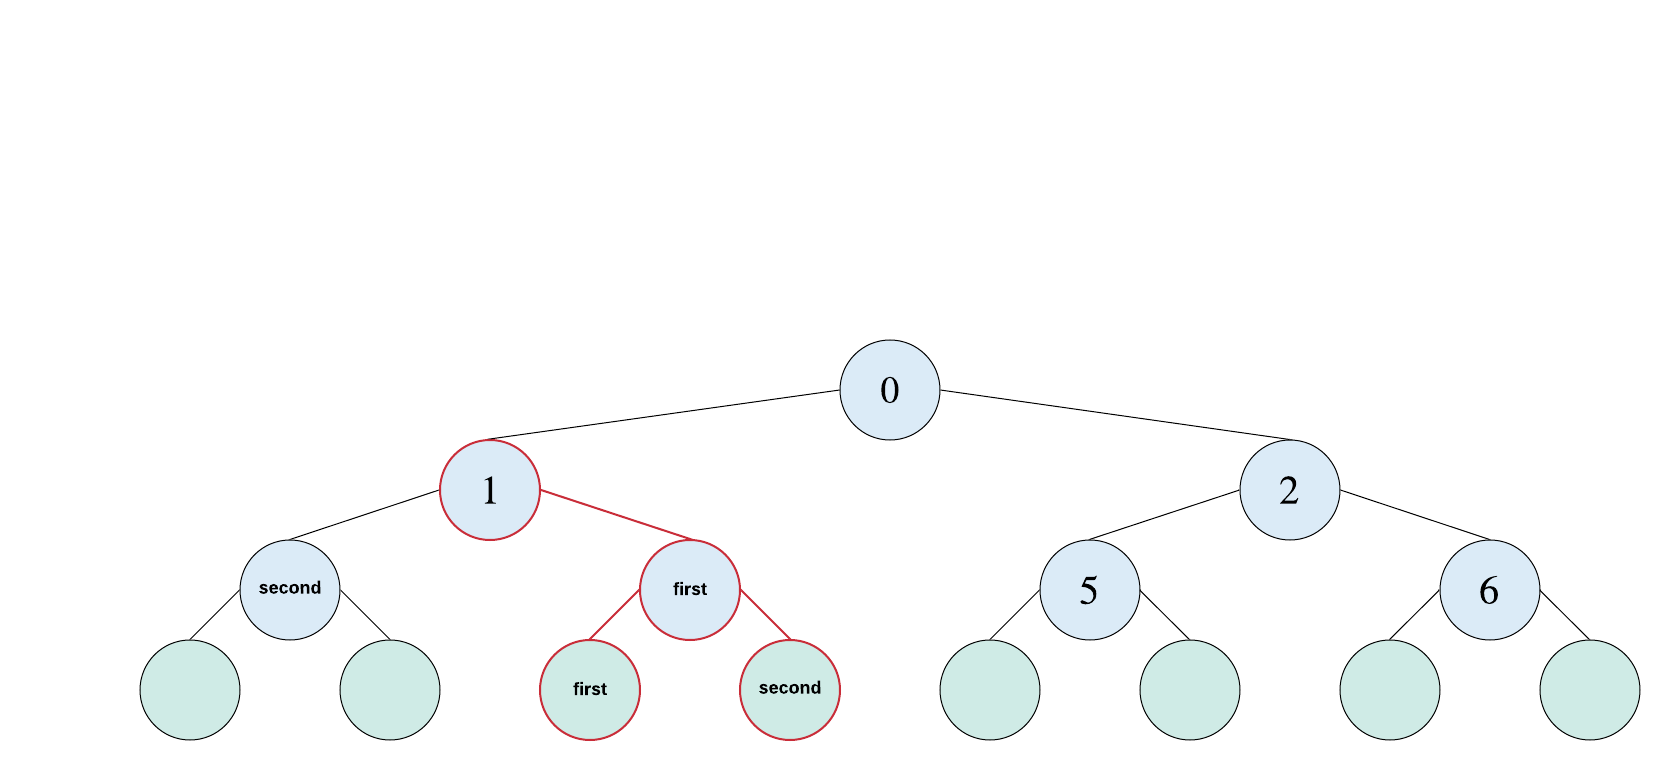
\includegraphics[width=0.9\textwidth]{pics/kd-tree-visual/5.png}
\caption{Visiting the second node of the initial leaf.}
\label{fig:t2}
\end{figure}

\noindent In figure \ref{fig:t3} the traversal looks to the parents second child, and since that has not yet been visited, it traverses to the first leaf of the parents second child.  

% \begin{figure}[H]
% \centering
% 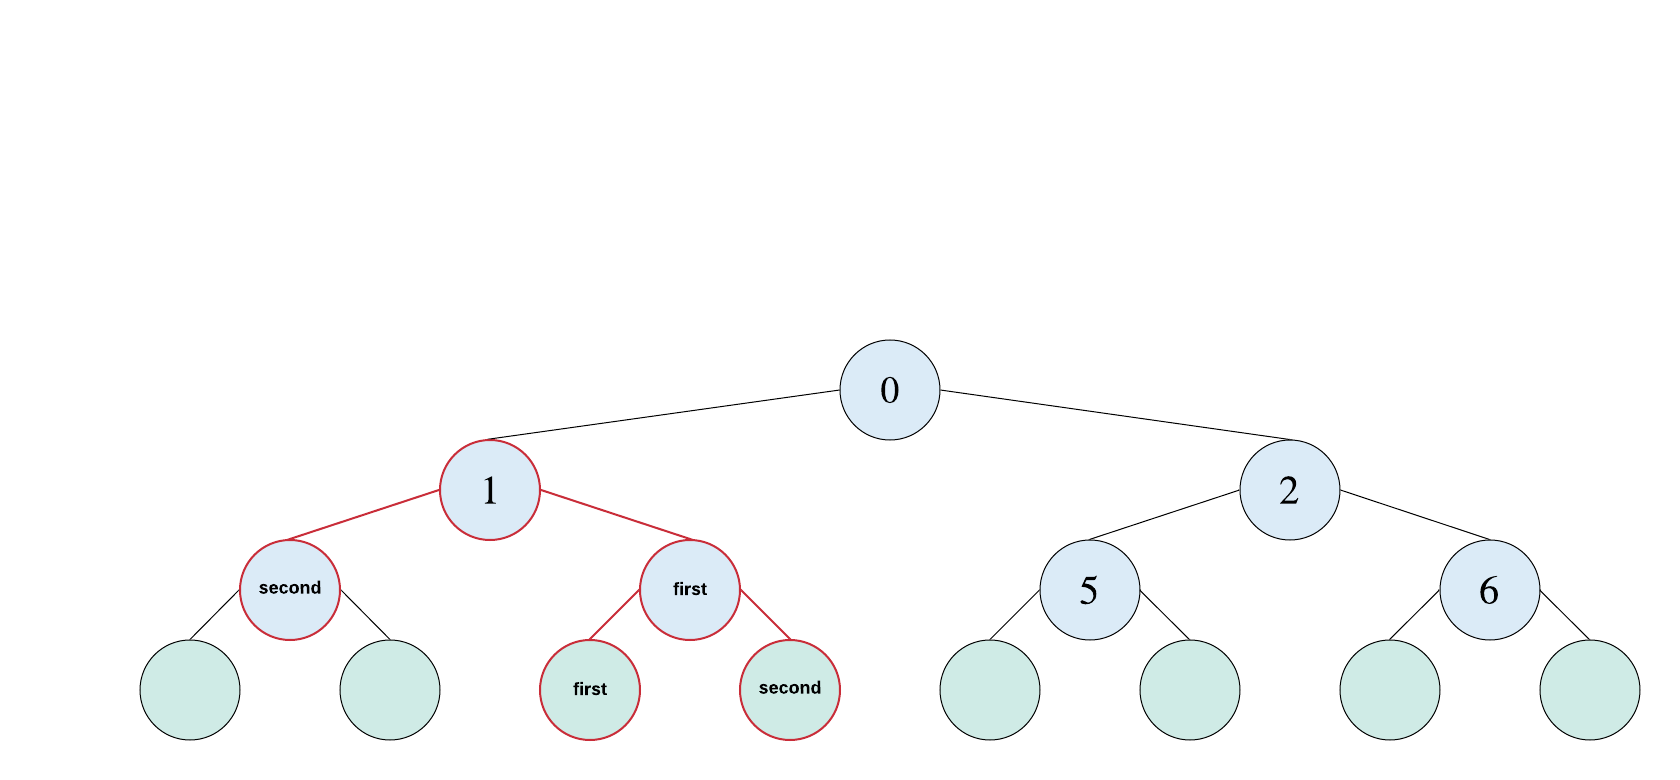
\includegraphics[width=0.9\textwidth]{pics/kd-tree-visual/6.png}
% \caption{}
% \end{figure}

\begin{figure}[H]
\centering
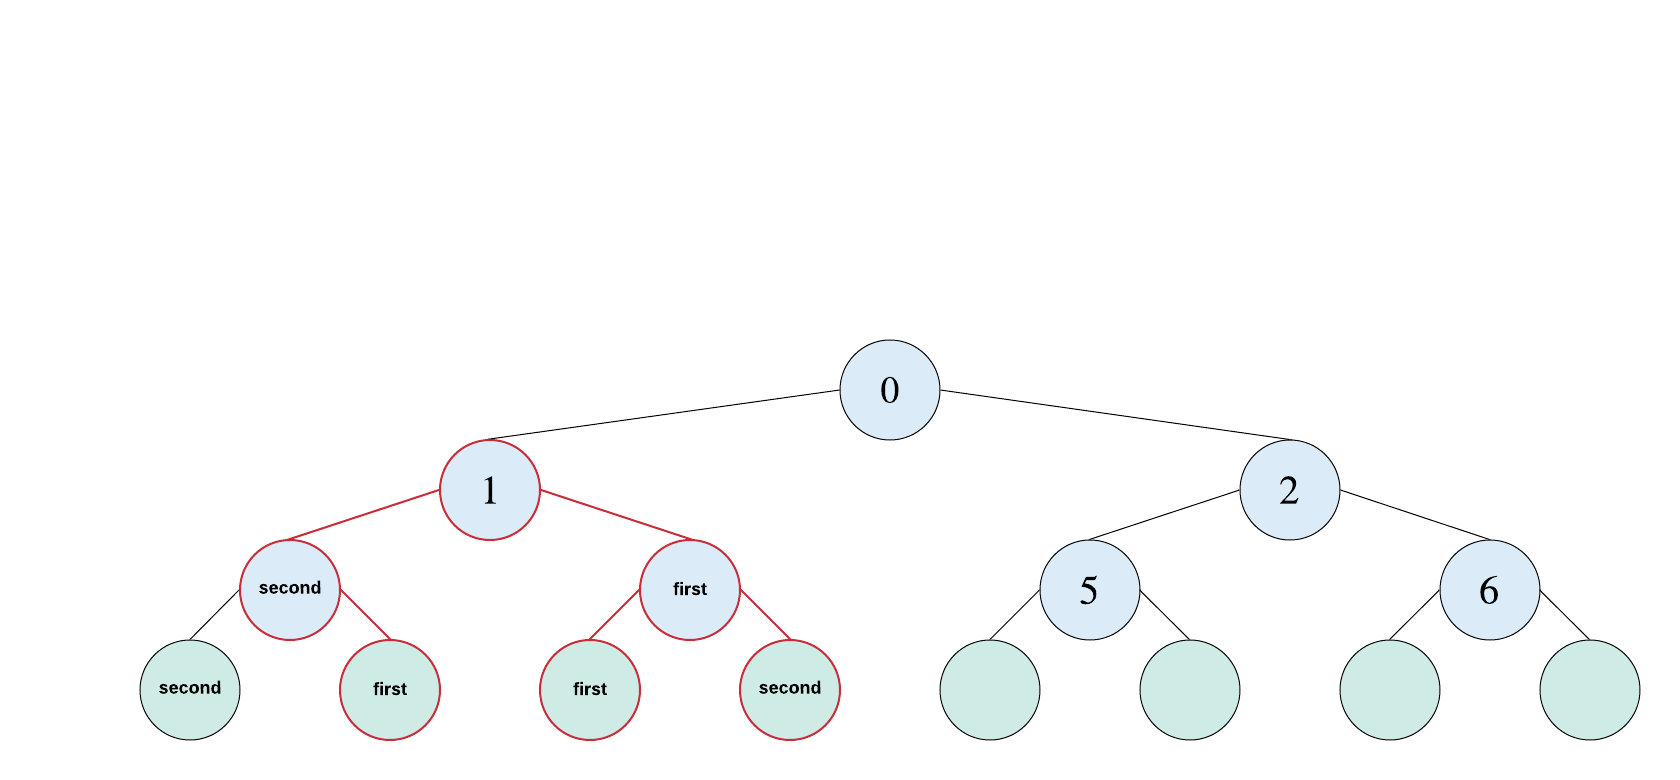
\includegraphics[width=0.9\textwidth]{pics/kd-tree-visual/7.png}
\caption{Visiting first node of the parents second child.}
\label{fig:t3}
\end{figure}

\noindent Pretending that we still have not found the KNN, the traversal will continue into the second leaf of the parents second child, as in figure \ref{fig:t5}. If the KNN is still not found, the traversal will continue to the second child of the root until the whole tree has been traversed, or the KNN is found. 

% \begin{figure}[H]
% \centering
% 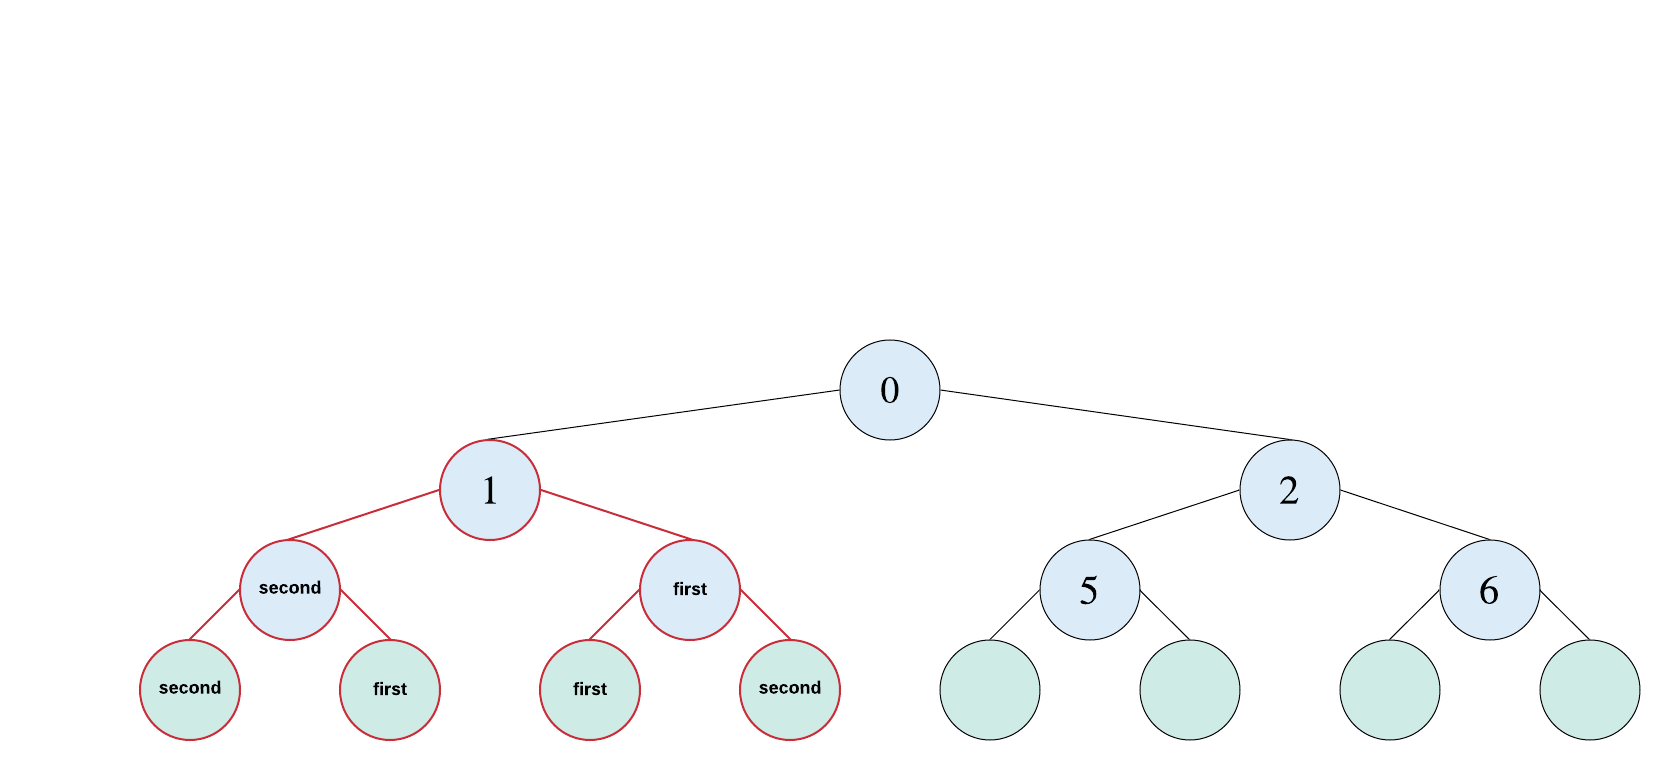
\includegraphics[width=0.9\textwidth]{pics/kd-tree-visual/8.png}
% \caption{}
% \end{figure}

% \begin{figure}[H]
% \centering
% 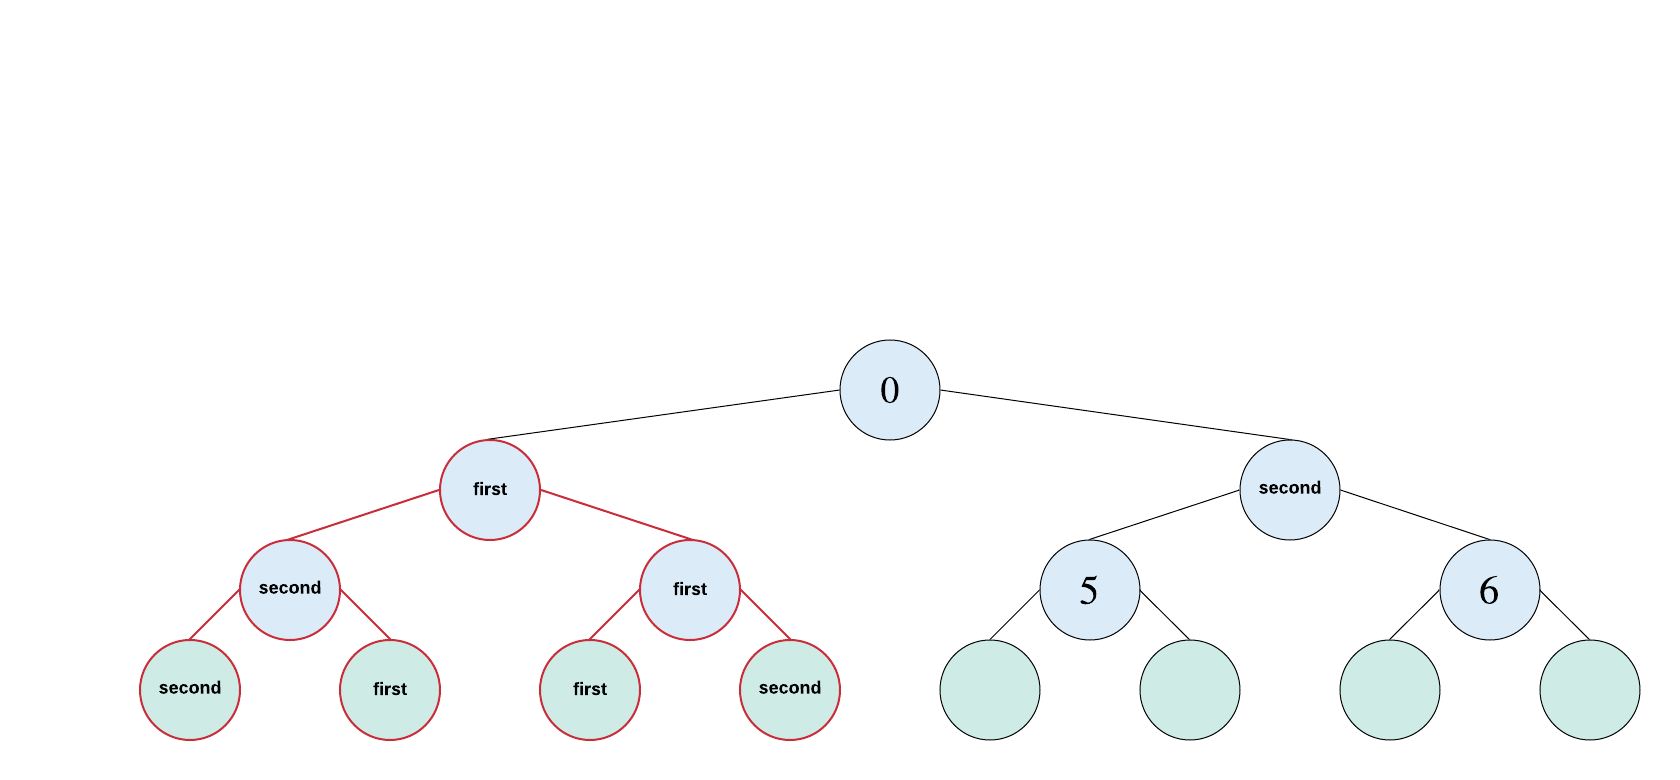
\includegraphics[width=0.9\textwidth]{pics/kd-tree-visual/9.png}
% \caption{}
% \end{figure}

% \begin{figure}[H]
% \centering
% 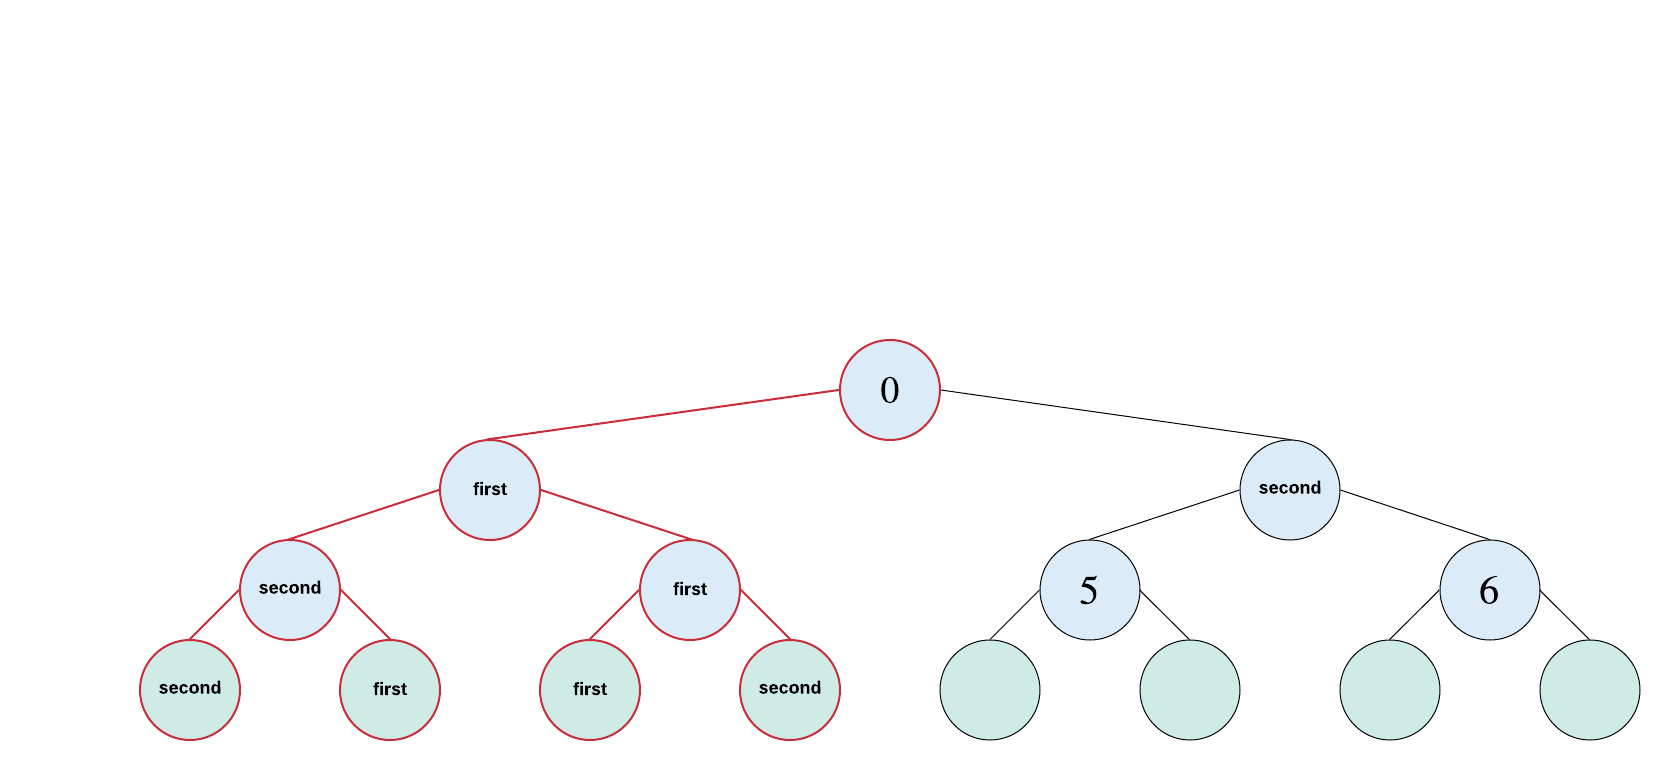
\includegraphics[width=0.9\textwidth]{pics/kd-tree-visual/10.png}
% \caption{}
% \label{fig:t4}
% \end{figure}

\begin{figure}[H]
\centering
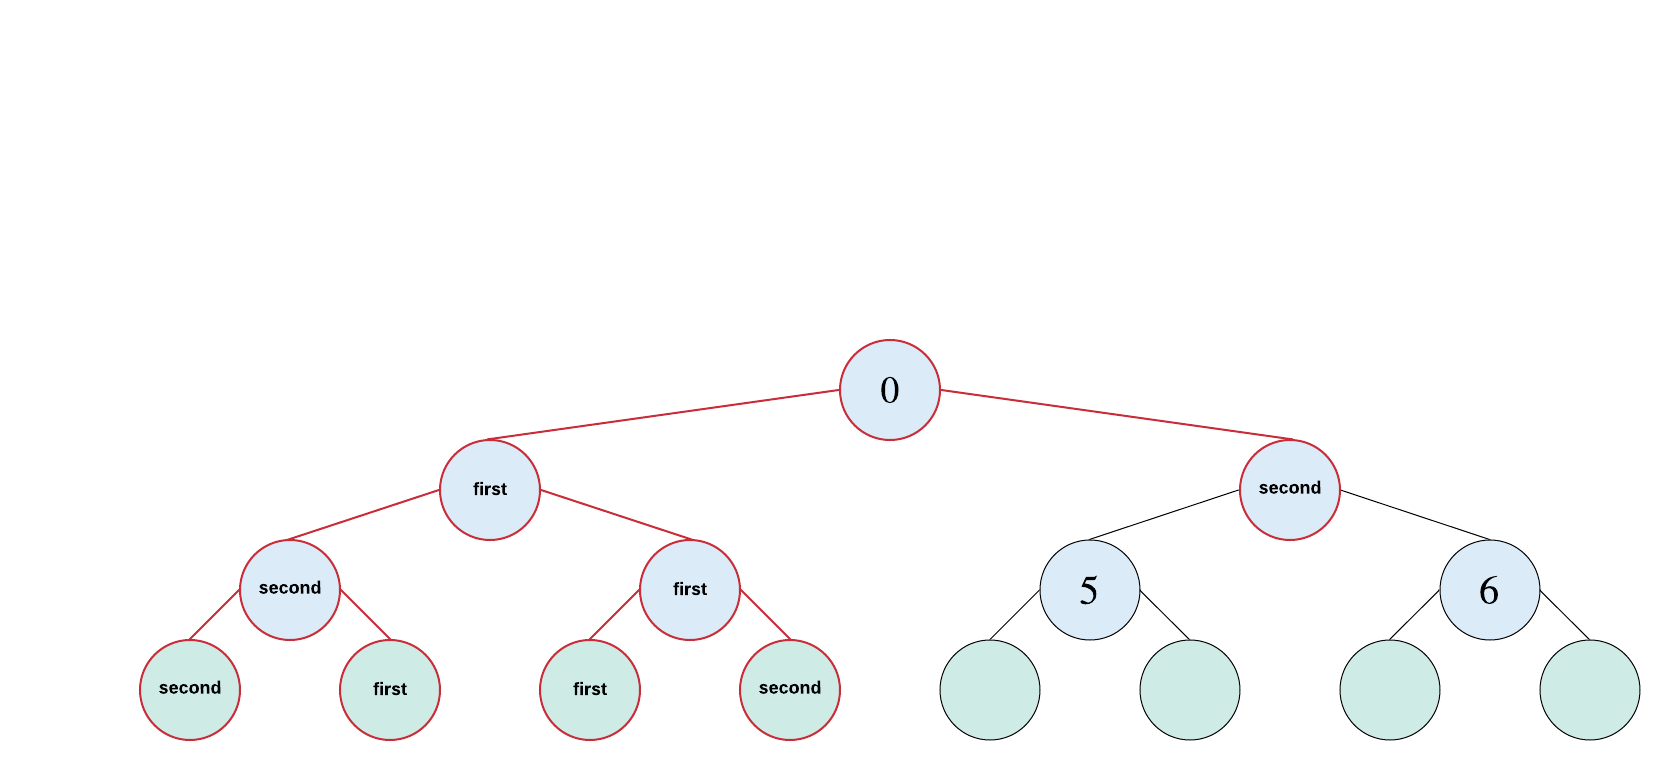
\includegraphics[width=0.9\textwidth]{pics/kd-tree-visual/11.png}
\caption{}
\label{fig:t5}
\end{figure}




% \subsubsection{Representing the Stack as an Integer}

%The naive solution of representing a stack is using a boolean list where the leaves and node are set to true once visited. Although this is a simple and correct solution, 
% The stack is represented as an integer, since the height of the tree never exceeds 32, making it is plausible. 
%it can be further optimised as an integer representation instead. % The code in listing XX shows the bit arithmetic done to modify the right areas of the stack and the logic behind setVisited is demonstrated in XX. 

% \begin{listing}[H]
% \begin{minted}{haskell}
%   let setVisited (stk: i32) (c: i32) : i32 =
%       stk | (1 << c)
%   let resetVisit (stk: i32) (c: i32) : i32 =
%       stk & !(1 << c)
%   let isVisited (stk: i32) (c: i32) : bool =
%       (stk & (1 << c)) > 0i32
% \end{minted}
% \caption{Snippet of bit arithmetic for stack modifications.}
% \label{lst:stack}
% \end{listing}

% \begin{figure}\label{fig:bits}
% \begin{align*}
%   && &00000000000000000000100010000101 &\\ \text{or} 
%   && &00000000000000000000001000000000 &\\ 
%   \cline{3-4}
%   && &00000000000000000000101010000101
% \end{align*}
% \caption{Example of stack integer arithmetic.}
% \end{figure}



% \begin{align*}
%   && &00000000000000000000101010000101 &\\ \text{and} 
%   && &11111111111111111111110111111111 &\\ 
%   \cline{3-4}
%   && &00000000000000000000100010000101
% \end{align*}







\subsubsection{Validating Whether to Look at the \texttt{second}}
\label{sec:valid}

We propose an optimised solution for checking whether to visit the second node or not. $wknn$ denotes the worst found neighbour so far, $R$ denotes our reference points, $Q$ denotes our queries, $lb$ and $ub$ denote the arrays containing the upper and lower bounds and $M$ denotes the array containing the median values for each node. 

\[
\forall i.[lb_i, ub_i].\ \forall q\in Q_m.\ \forall p\in R_n.\ \forall m\in M_{nn}.
\]

\noindent The original solution determines whether to visit the second node by checking if the distance from the query to the current median is smaller than the worst found neighbour, as in Equation \ref{eq:e1}. However, the solution looks only at one dimension when checking whether to visit or not, meaning that it is likely that another dimensionality could contain information that would otherwise have prevented the second visit. Especially if the number of dimensions is, because then a lot of values will be overlooked. 
% The original solution looks at one dimension when checking whether to visit the second node or not.

\begin{equation}  \label{eq:e1}
\mid q_i - m_i \mid\ >\ wknn
\end{equation} 

\noindent The naive approach would be to compute all distances, as in Equation \ref{eq:e2}. Although this has a higher level of accuracy compared to the original solution, it also inefficient. 

\begin{equation}  \label{eq:e2}
% \substack{ \forall i.[lb_i, ub_i]. \\ \forall q\in Q_m. \\ \forall p\in R_n.} \ 
\sqrt{ \sum_{i}^{} (p_i - q_i)^2  }
\ \geq\ wknn
\end{equation}

\noindent Instead, we propose a solution that achieves a higher level of accuracy compared to the original solution, while still running efficiently. The idea is that the upper and lower bounds for each dimension is saved, for each node, and then used to compute the distance between the query to the upper and lower bounds, respectively. Thus, instead of checking one dimension, we check all dimensions, but only against the upper and lower bounds. This is formulated in Equation \ref{eq:e3} and it corresponds to lines 11-26 in Listing \ref{lst:traverse1}. 

\begin{equation}  \label{eq:e3}
% \substack{ \forall i.[lb_i, ub_i]. \\ \forall q\in Q_m. \\ \forall p\in R_n.} \ 
\sqrt{ \sum_{i}^{} (p_i - q_i)^2  }\ \geq\
\sqrt{\sum_{i}^{} \substack{(q_i-lb_i)^2 \\ (q_i-ub_i)^2 \\\text{  ~ ~ ~   }0}  \substack{\text{, if  ~ } q_i\ \leq\ lb_i \\ \text{, if  ~ } q_i\ \geq\ ub_i \\\text{, ~ otherwise} }}
\ \geq\ wknn
\end{equation}

\noindent Section \ref{sec:evaltrav} demonstrates the increased performance by using this solution. On a dataset of size roughly 4 mio., with dimensionality D=12 and K=5, we obtain a speed-up of $5.6$. The reason for this is elaborated further in Section \ref{sec:evaltravhist}, which demonstrates how the checking all the upper and lower bound on all dimensions reduces the number of visits to additional node, due to its increased accuracy. Thus, reducing the steps made in the traversal and improving the performance. 


\begin{listing}[H]
\begin{minted}{haskell}
  let (parent_rec, stack, count, rec_node) =
      loop (node_index, stack, count, rec_node) =
           (last_leaf, stack, height, -1)
            while (node_index != 0) && (rec_node < 0) do
                let parent = getParent node_index
                let second = node_index + addToSecond node_index in

                if isVisited stack count
                then (parent, stack, count-1, -1)
                else
                  let ack = loop ack = 0.0f32
                      for i < d do
                          let cur_q = query[i]
                          let lower = lower_bounds[second,i]
                          let upper = upper_bounds[second,i] in

                          if cur_q <= lower then
                              let res = (cur_q-lower)*(cur_q-lower)
                              in (ack + res)
                          else if cur_q >= upper then
                              let res = (cur_q-upper)*(cur_q-upper)
                              in (ack + res)
                          else (ack + 0.0)

                  let to_visit = (f32.sqrt ack) < wknn in
                  if !to_visit
                  then (parent, stack, count-1, -1)
                  else
                    let second = node_index + addToSecond node_index
                    let stack  = setVisited stack count in
                    (parent, stack, count, second)
\end{minted}
\caption{A part of the tree traversal demonstrating checking upper and lower bound to determine visits.}
\label{lst:traverse1}
\end{listing}


% \[
%   \sum_{i}^{} \substack{(q_i-lb_i)^2, if  q_i \leq lb_i \\ (q_i-ub_i)^2, if  q_i \geq ub_i \\0 , otherwise }
% \]

% \begin{equation}
%   \sqrt{\sum_{i}^{} \substack{(q_i-lb_i)^2 \\ (q_i-ub_i)^2 \\\text{  ~ ~ ~   }0 }  \substack{\text{, if  ~ } q_i\ \leq\ lb_i \\ \text{, if  ~ } q_i\ \geq\ ub_i \\\text{, ~ otherwise} }}
% \end{equation}

% \[
%   \sum_{\substack{i=0 \\ i\neq 4}}^n \substack{i=0 \\ i\neq 4}
% \]


% \[
% \mathit{dist} = 
% \sqrt{ \left( \frac{dx}{hx} \right)^{\!\!2} +  \left( \frac{dy}{hy} \right)^{\!\!2} +  \left( \frac{dz}{hz} \right)^{\!\!2}}
% \]


% \begin{listing}[H]
% \begin{minted}{haskell}
% entry traverse [d][n][l] (height:             i32)  (median_dims:     [n]i32)
%                          (median_vals:     [n]f32)  (wknn:               f32)
%                          (query:           [d]f32)  (stack:              i32) 
%                          (last_leaf:          i32)  (lower_bounds: [l][d]f32)
%                          (upper_bounds: [l][d]f32)  : (i32, i32) =

%   (...) -- stack functions for checking and setting the stack

%   let (parent_rec, stack, count, rec_node) =
%       loop (node_index, stack, count, rec_node) =
%            (last_leaf, stack, height, -1)
%             while (node_index != 0) && (rec_node < 0) do
%                 let parent = getParent node_index
%                 let second = node_index + addToSecond node_index in

%                 if isVisited stack count
%                 then (parent, stack, count-1, -1)
%                 else
%                   let ack = loop ack = 0.0f32
%                       for i < d do
%                           let cur_q = query[i]
%                           let lower = lower_bounds[second,i]
%                           let upper = upper_bounds[second,i] in

%                           if cur_q <= lower then
%                               let res = (cur_q-lower)*(cur_q-lower)
%                               in (ack + res)
%                           else if cur_q >= upper then
%                               let res = (cur_q-upper)*(cur_q-upper)
%                               in (ack + res)
%                           else (ack + 0.0)

%                   let to_visit = (f32.sqrt ack) < wknn in
%                   if !to_visit
%                   then (parent, stack, count-1, -1)
%                   else
%                     let second = node_index + addToSecond node_index
%                     let stack  = setVisited stack count in
%                     (parent, stack, count, second)

%   let (new_leaf, stack, _) =
%       if parent_rec == 0 && rec_node == -1 then
%            (-1, stack, 0)

%       else loop (node_index, stack, count) =
%                 (rec_node, stack, count)
%            while !(isLeaf height node_index) do
%               let count = count + 1
%               let stack = resetVisit stack count in
%               if query[median_dims[node_index]] <= median_vals[node_index]
%               then ((node_index+1)*2-1, stack, count)
%               else ((node_index+1)*2, stack, count)

%   in (new_leaf, stack)
% \end{minted}
% \caption{Futhark implementation of the tree traversal.}
% \label{lst:traverse}
% \end{listing}





% \subsubsection{Difficulties and Shortcomings}







































